\subsection{Особенности электронного и геометрического строения олефиновых комплексов, по сравнению с карбонильными. Модель Дьюара-Чатта-Дункансона}

\subsubsection*{Строение олефиновых комплексов на примере соли Цейзе}: 
$$[PtCl_4]^{2-} + EtOH => [Pt(C_2H_4)Cl_3] + Cl^- + H_2O$$

\begin{figure}[htp]
\centering
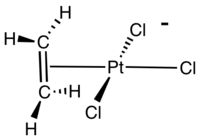
\includegraphics[scale=1.00]{/home/someanonimcoder/TeX/tic_summer/images/ceise.png}
\end{figure}

Ось связи $CC$ перпендикулярна комплексу.

Между молекулой этилена и центральным атомом - боковая дативная связь: частичная передача электронной плотности с $\pi$-орбитали лиганда на вакантнуюорбиталь M и с заполненной d-АО M на вакантную $\pi^*-L$.

\begin{itemize}
	\item Высокое сродство к электрону металла увеличивает $\sigma-$донирования $M->olephine$ 	в химическую связь
	\item Низкое значение энергии возбуждения увеличивает вклад $\pi-$компоненты $M->olephine$
	\begin{itemize}
		\item Ni: $PE=1.72eV$, $d^{10}$, $E_A = 1.20eV$ - хороший $\pi-$донор
		\item Hg: $PE=12.8eV$, $d^{10}$, $E_A = 16.9eV$ - 	хороший $\pi-$акцептор
		\item Pd: $PE=3.05eV$, $d^{8}$, $E_A = 18.56eV$ - хороший $\pi-$донор и $\pi-$акцептор
	\end{itemize}
	\item Олефин способен сохранить как в роли кислоты, так и основания Льюиса, тем самым сохраняя низкую полярность связи.
	\item Энергия связи $M-$олефин определяется вкладом обр. $\pi-$донирования.
\end{itemize}

\subsubsection*{Модель Дьюара-Чатта-Дункансона}

Данная модель рассматривает оба механизма - как прямое, так и обратное донирование. От того, какие заметсители и лиганды есть у олефина и лиганда соответственно, зависит то, какой из механизмов будет преобладать:

\begin{itemize}
	\item Донорные заместители у олефина - увеличивают вклад $\pi-olefine => d-Me$
	\item Акцепторные заместители у олефина - увеличивают вклад $d-Me => \pi^*-olefine$
	\item Акцепторные лиганды металла - увеличивают вклад $\pi-olefine => d-Me$
	\item Донорные лиганды у металла - увеличивают вклад $d-Me => \pi^*-olefine$
\end{itemize}






